\section{Introduction}\label{sec:intro}
%\todo[inline]{basic history of development of neuro-type models and how they have increased in complexity. The probelms with parameters derived from experiments (different animals etc, the lack of information on error tolerances) }
%During the last two decades \gls{fmri} has proven to be an established tool in studying the human brain. This is especially true in the case of the \gls{bold} signal, where changes in blood oxygen levels can be detected via the magnetic signal  \cite{Ogawa1990}. However due to the constraint on the resolution of \gls{bold}, \gls{fmri} methodology has not been used extensively to study the underlying cellular neural architecture and their associated cerebral functions. Complex models that address this important relationship and constructing a detailed compartmental model with the relevant cell types involved will allow simulations relating certain brain functions performed in a region to its \gls{fmri} \gls{bold} response. The \gls{nvc} mechanism, the cerebral metabolic rate of oxygen consumption, and the \gls{cbv} are known to contribute to the \gls{fmri} \gls{bold} response \citep{Buxton2004}, however a thorough understanding of these factors has yet to be fully established.
Over the past 20 years the use of computational models to describe physiological phenomena has grown almost exponentially. This growth has clearly provided significant advantages to the experimental community in that it can furnish results of ''\textit{in-silico}'' experiments which are either ethically or physically impossible in the laboratory. However there is always a downside to progress and in this case the models have, (for a variety of reasons, most notably the requirement that the models should possess complex cellular functions which are thought \textit{but not necessarily proven} to be important ) increased in their complexity with a concomitant increase in the associated parameters. These parameters, in defining the relevant phenomenon, more often than not come from a plethora of animal experiments whose relationship to the human physiology is weak to say the least, but in the large majority of cases that is all that is available.  In addition experimental results in the public domain provide very little information on the errors in these measurements. It is important to recognise that we differentiate between variations in experimental results between animals of the same type (derived from the same experiment) and the actual error in measurement. \\

Physiological models, even those of a simple form are highly non-linear, requiring very careful analysis if they are to be useful. For large complex systems it is unclear as to the sensitivity of parameters to the numerical production of phenomena. Herein lies one of the diffculites of modelling, what effect do the errors in parameters determined from experiment have on the output of a non-linear numerical model? Compounded by complexity and the large dimension in which the numerical solution is analysed, sensitivity analyses requires not only computationally expensive resources but also robust analytical tools that can operate within the dimension determined by the vector of parameters. Importantly in analysing this sensitivity we can learn significant facts about the physiology of the system which would have stayed hidden under the premice of simply producing results.  \\

In this context we investigate the sensitivity of a complex physiological system (defined below), which has a large parameter dimension where most (if not all) of the parameter values come from non-human experiment  with an inherent (unknown) error.

\subsection{Physiological Model: Neurovascular Coupling}
The \gls{nvc} response, the ability to locally adjust vascular resistance as a function of neuronal activity, is believed to be mediated by a number of different signalling mechanisms. \citet{Roy1890} first proposed a  mechanism based on a metabolic negative feedback theory. According to this theory, neural activity leads to a drop in oxygen or glucose levels and increases in CO$_2$, adenosine, and lactate levels. All of these signals could dilate arterioles and hence were believed to be part of the neurovascular response. However, recent experiments illustrated that the \gls{nvc} response is partially independent of these metabolic signals \citep{Leithner2010, Lindauer2010, Mintun2001, Powers1996, Makani2010}. An alternative to this theory was proposed where the neuron releases signalling molecules to directly or indirectly affect the blood flow. Many mechanisms such as the \gls{pot} signalling mechanism \cite{Filosa2006}, the \gls{no} signalling mechanism or the arachidonic acid to \gls{eet} pathway are found to contribute to the neurovascular response \citep{Attwell2010}.

The \gls{pot} signalling mechanism of \gls{nvc} seems to be supported by significant evidence, although new evidence shows that the endfoot astrocytic \gls{ca} could play a significant role. The \gls{pot} signalling hypothesis mainly utilises the astrocyte,  positioned to enable the communication between the neurons and the local perfusing blood vessels. The astrocyte and the \glspl{ec} surrounding the perfusing vessel lumen exhibit a striking similarity in ion channel expression and thus can enable control of the \gls{smc} from both the neuronal and blood vessel components \citep{Longden2015}. Whenever there is neuronal activation \gls{pot} ions are released into the \gls{ecs} and \gls{sc}. The astrocyte is depolarised by taking up \gls{pot} released by the neuron and releases it into the \gls{pvs} via the endfeet through the BK channels \citep{Filosa2007}. This increase in \gls{ecs} \gls{pot} concentration ($3-10$ mM) near the arteriole hyperpolarises the \gls{smc} through the \gls{kir} channel, effectively closing the voltage-gated \gls{ca} channel, reducing smooth muscle cytosolic \gls{ca} and thereby causing dilation. Higher \gls{pot} concentrations in the \gls{pvs} cause contraction due to the reverse flux of the \gls{kir} channel \citep{Farr2011}. 

Amidst the difficulty in monitoring and measuring the rapid changes in metabolic demands in the highly heterogeneous brain, speculative estimates of the relative demands of the cerebral processes that require energy were given based on different experimental data by \citet{Ames2000}. As per the estimate, the vegetative processes that maintain the homeostasis including protein synthesis accounted for $10-15$\% of the total energy consumption. The costliest function seems to be in  restoring the ionic gradients during neural activation. The \gls{sodpot} exchange pump is estimated to consume $40-50$\%, while the \gls{ca} influx from organelles and extracellular fluid consumes $3-7$\%. The processing of neurotransmitters such as uptake or synthesis consumes $10-20$\%, while the intracellular signalling systems which includes activation and inactivation of proteins consumes $20-30$\%. The rest of the energy is estimated to be consumed by the axonal and dendritic transport in both directions.

Previous work \cite{Mathias2018} has provided  the construction of an experimentally validated numerical (\textit{in silico}) model based on experimental data to simulate the \gls{fmri} \gls{bold} signal associated with \gls{nvc} along with the associated metabolic and blood volume responses. An existing neuron model \citep{Mathias2017, Mathias2017a} has been extended to include an additional transient \gls{na} ion channel (NaT) expressed in the neuron, and integrated into a complex \gls{nvc} model \citep{Dormanns2015, Dormanns2016, Kenny2017a}. This present model is based on the hypothesis that the \gls{pot} signalling mechanism of \gls{nvc} is the primary contributor to the vascular response and the \gls{sodpot} exchange pump in the neuron is the primary consumer of oxygen during neural activation. The model contains some 317 parameters, most of which come from non-human experiments and some are fundamental such as Faraday's constant. We have chosen a subset of the parameter vector which defines pathways that are considered important for the normal function of neurovscular coupling. The subset for which we constrain the parameters to be constant rather than have a pdf define leak terms, characteteristic oxygen and other species concentrations, buffer concentrations, volume surface ratios etc. The subset for which we do provide ramdom variability is based on the work by \cite{Dormanns2016} and \cite{Kenny2018}. These works investigate basic pathways such as the nitric oxide and potassium. By providing ramdom variablity to parameters that support these pathways the dimension of the subset is redeuced from 317 to 160. Clearly the algorithms defined below can be used to investigate other areas of interest for any complex model including that of neurovascular coupling. However for this initial work we constrain ourselves to the above subset. 
Figure \ref{fig:nvu20} shows the components and main pathways of the neurovascular coupling model (version 2.0) \\
We wish to analyse parameter sensitivity with respect to certain conditions and/or phenomena that occur during neurovascular coupling. From previous work it is known that the \pot concentration in the extracellular space (ECS) is crucial to maintaining a homeostatic state (large concentrations of \pot support the propagation of spreading depression waves) hence we choose to look at the mena value of \pot in the ECS. Secondly neurovascular coupling is the main phenomenon providing oxygen and nutrients to the neuronal tissue. This is mediated by the local arteriole dilating and (under the assumption of constant pressure) increasing the flow of blood into the tissue. We therefore define the time averaged cerebral blood flow determined over the course of neuronal stimulation. The contraction/dilation of the arteriolar vessel  depends on the smooth muscle cell (SMC) concentration of \ca and the phophorylation of the actin/myocin complex. Our third Quantity of Interest (QoI) is the minimum combined concentration of the actin myosin complex, both phosphorylated and unphosphorylated. This allows us to analyse the functioning of the main components of the neurovascular unit (NVU) defined as the linked components of neuron, synaptic ceft, astrocyte, perivascular space (PVS), SMC, endothelial cell (EC), lumen (LU, the domain in which blood flows) and the ECS. 

\begin{figure}[h!]
\centering
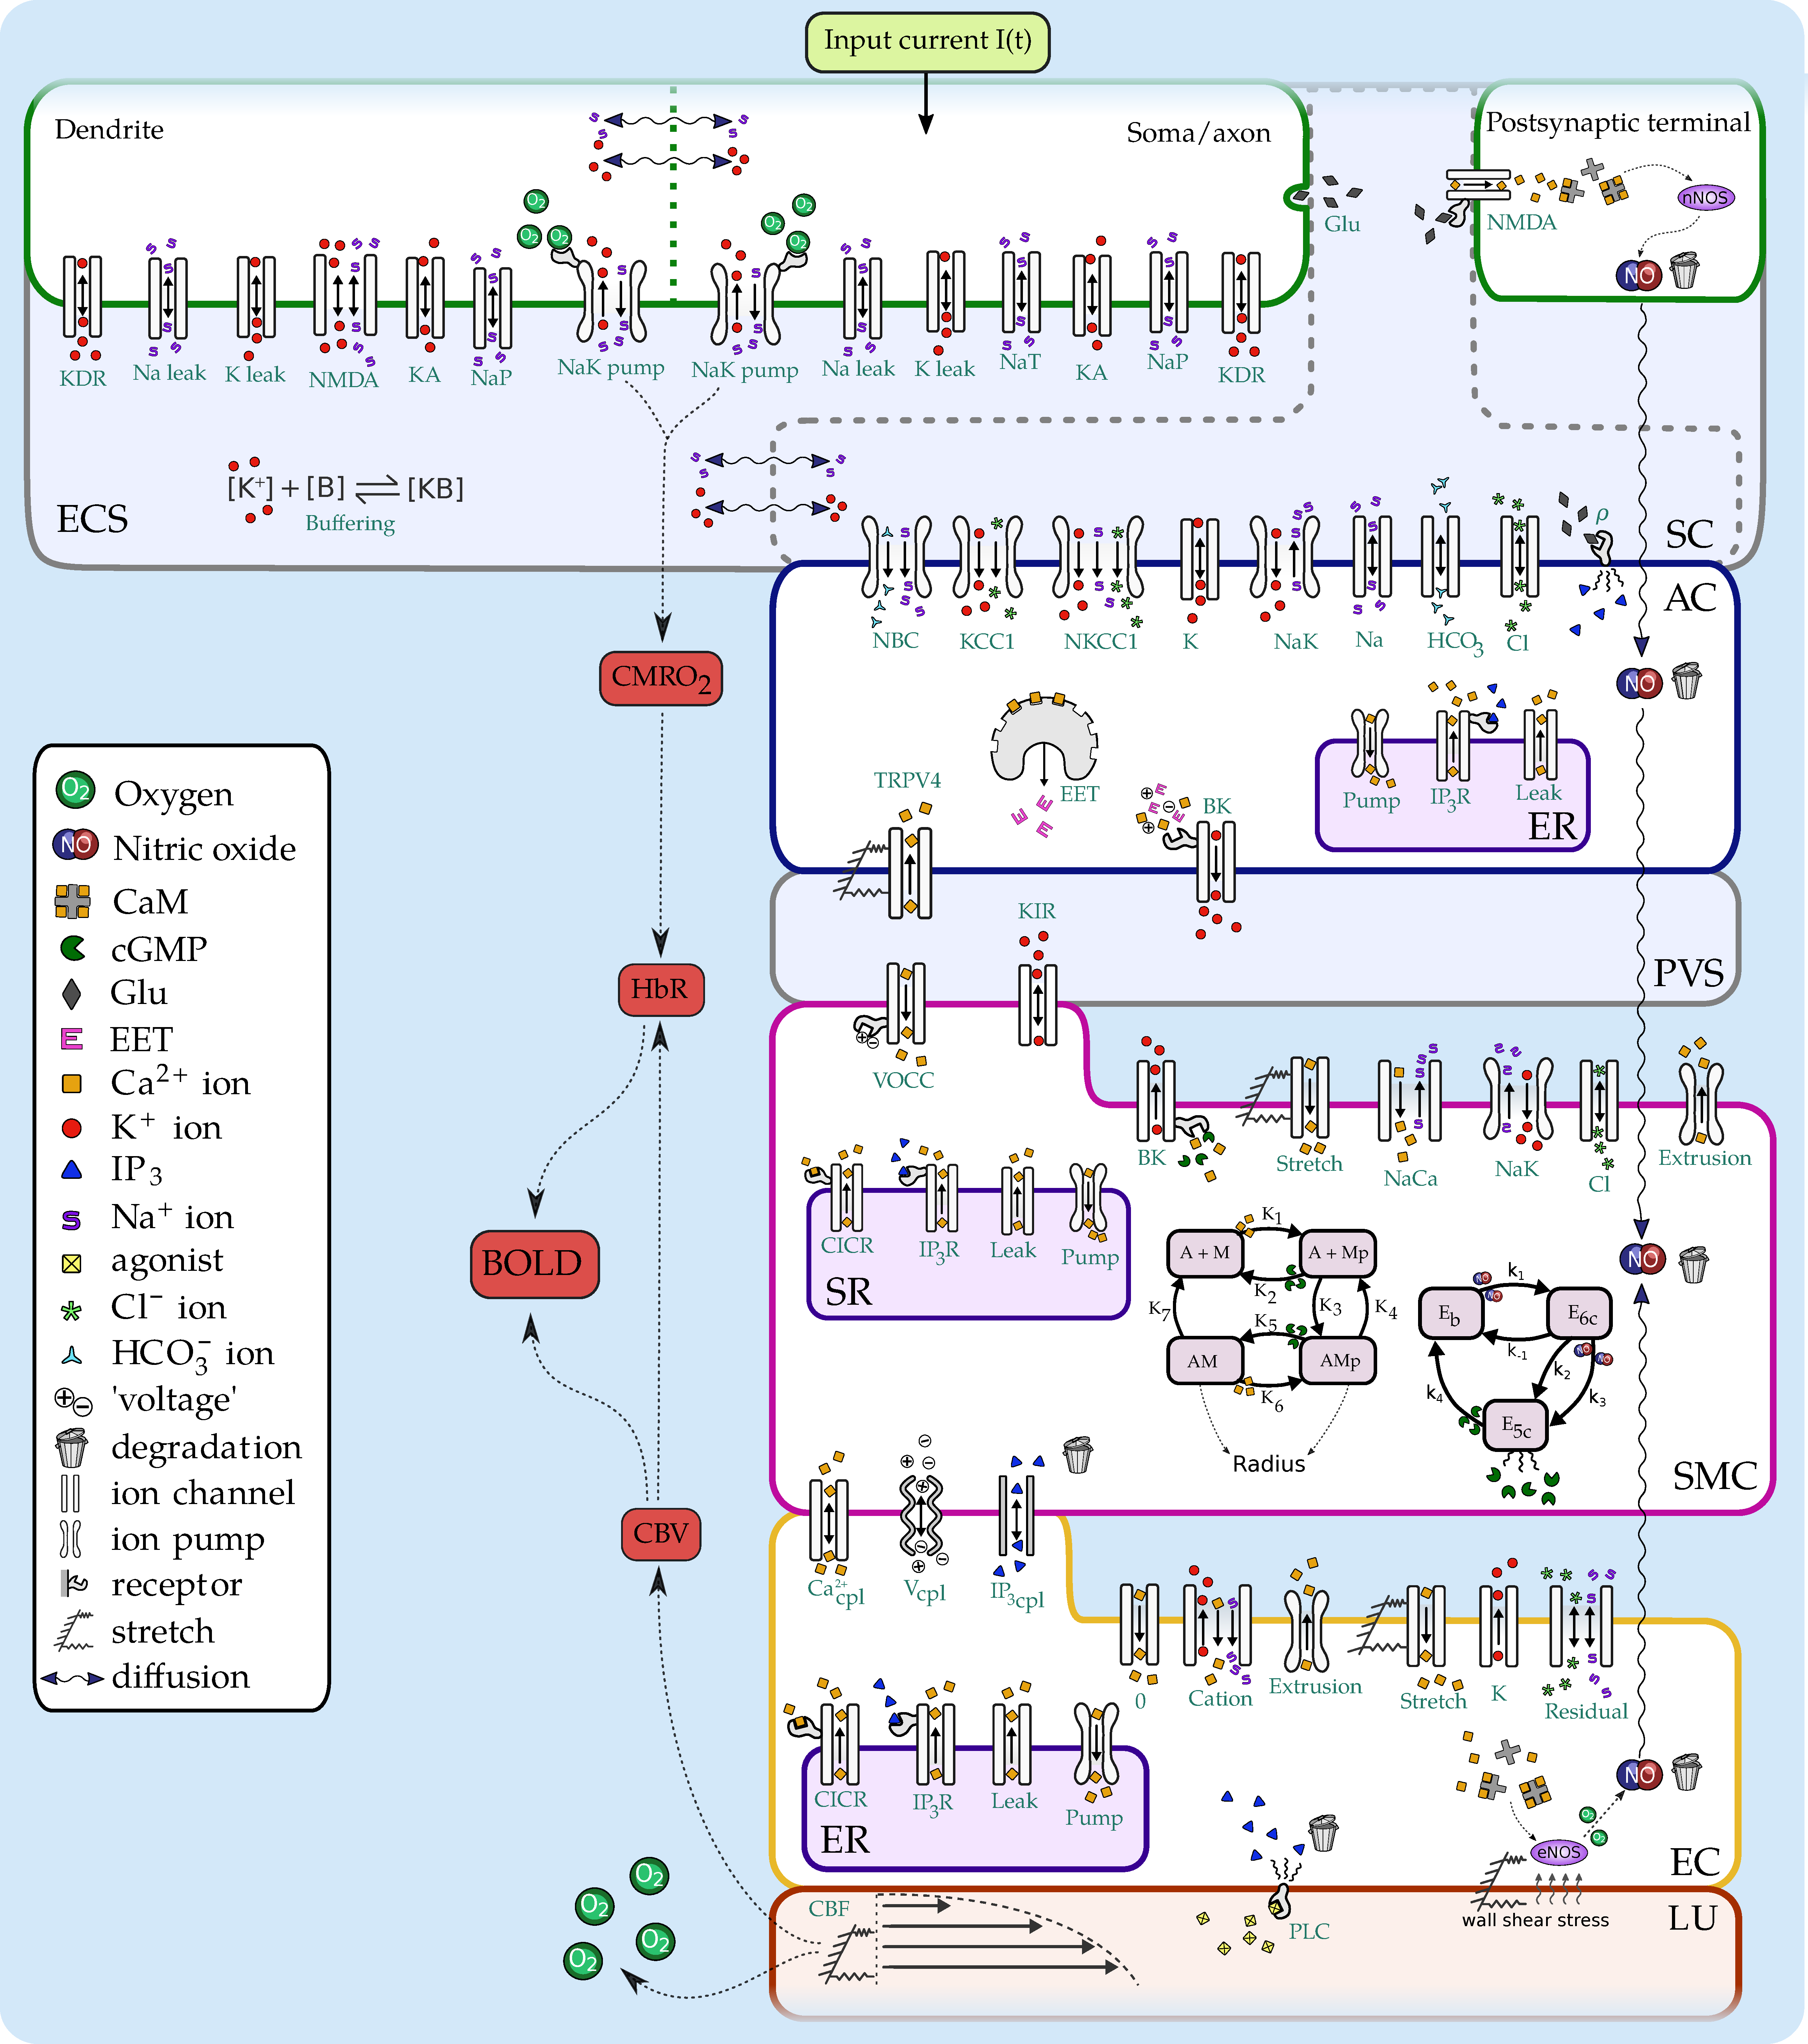
\includegraphics[width=0.7\linewidth]{Figures/nvu_20}
\caption[Graphic Sketch of NVU version 2.0]{Graphic Sketch of NVU version 2.0, showing the basic components of neuron, astrocyte, smooth muscle cell, endothelial cell, lumen and extracellular space. ion channels, pumps and pathways from neuron to endothelial cell are also shown in addition to the basis for evaluation of the fMRI blood oxygenation level signal (BOLD) protocol.}
\label{fig:nvu20}
\end{figure}

Such a complex model constructed with a high-dimensional parameter space is not easily amenable to sensitivity analyses considering the significant computing resource required. In fact, part of our contribution in this paper is to show how to meaningfully reduce the dimension of the original problem to make it amenable to standard Global Sensitivity Analysis (GSA) methods; the large dimension of the parameter space and the complexity of the model precludes the  direct application of GSA tools.
From a purely physiological perspective an understanding of the dominant cellular mechanisms resulting in cerebral tissue perfusion after neuronal stimulation would be of particular and important interest.\\
Previous work, both experimental and numerical about the function of neurovascular coupling provides data from which quantities of interest (QoIs) can be characterised. In this presented case we choose three which are defined above and in mathematical form in Section~\ref{sec:meth}. 

%\todo[inline]{state the reasons why we are doing this particular work. } 
%\todo[inline]{state reasons why we have chosen the specific QoIs} 
 % We have used the \gls{cbf} change from the experimental data \cite{Zheng2010} taken from the rat barrel cortex. 
  
 \todo[inline]{INTRODUCE NOTATION AND TERMINOLOGY WE CAN REFER TO THROUGHOUT THE ARTICLE}
  
Here are a few references we may consider citing  \cite{gsa_pharm,lr_gsa,uqpy,Witthoft2013}.
